\documentclass[tikz]{standalone}
\begin{document}

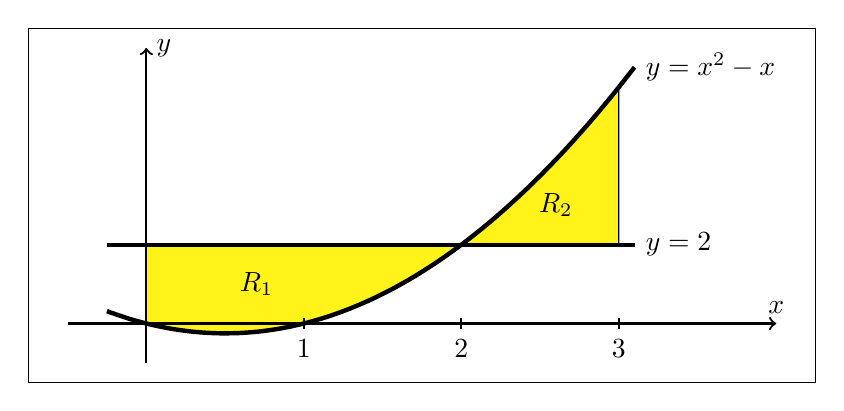
\begin{tikzpicture}[xscale=2.0,yscale=0.5]

  \draw[fill=white] (-0.75,-1.5) rectangle ++(5,9);

  % shade region
  \draw[fill=yellow!90] (0,2) -- plot[domain=0:3,smooth,variable=\x,black] ({\x},{\x* (\x -1)}) |- (0,2);

  % draw axes
  \draw[thick,->] (-0.5,0) -- (4,0) node[above] {$x$};
  \draw[thick,->] (0,-1) -- (0,7) node[right] {$y$};

  % draw curves
  \draw[ultra thick,domain=-0.25:3.1,smooth,variable=\x,black] plot ({\x},{\x* (\x -1)}) node[right] {$y=x^2-x$};
  \draw[ultra thick,domain=-0.25:3.1,smooth,variable=\x,black] plot ({\x},{2}) node[right] {$y=2$};
  %\draw[ultra thick,domain=-2.3:2.3,smooth,variable=\x,black] plot (\x,\x*\x*\x) node[right] {$y=x^3$};


  \draw (0.7, 1) node {$R_1$};
  \draw (2.6, 3.0) node {$R_2$};
        
  % tick marks
  \foreach \x in {1,2,3} 
    \draw [thick] (\x cm,4pt) -- (\x cm,-4pt) node[below] {$\x$};

\end{tikzpicture}
\end{document} 
